\documentclass[aps,pre,reprint,longbibliography,nofootinbib,floatfix]{revtex4-2}
\usepackage[T1]{fontenc}
\usepackage{amsmath,amssymb}
\usepackage{graphicx}
\usepackage{booktabs}
\usepackage{fancyvrb}
\usepackage[colorlinks=true,allcolors=blue]{hyperref}
\hypersetup{pdftitle={Activity above one half in finite Glauber annealing},
pdfauthor={Xiaojian Zeng},pdfsubject={Finite-state nonequilibrium Glauber dynamics}}
\newcommand{\Act}{\mathcal A}
\newcommand{\eps}{\epsilon}
\renewcommand{\topfraction}{0.95}
\renewcommand{\bottomfraction}{0.95}
\renewcommand{\textfraction}{0.05}
\begin{document}
\title{Activity above one half in finite Glauber annealing}
\author{Xiaojian Zeng}
\email{xiaojianzeng@foxmail.com}
\affiliation{PBC School of Finance, Tsinghua University, 100190}
\date{September 12, 2026}
\begin{abstract}
The equilibrium jump probability of a heat-bath Glauber update on a regular
state graph is at most one half. We give a finite counterexample to extending
this bound to arbitrary monotone cooling from a Gibbs initial state.
An eleven-state, four-regular graph and a two-update cooling schedule at
strictly positive, finite temperatures give a second-step activity greater than $63/125$ and
a two-step mean greater than $251/500$. All sign decisions reduce to exact
rational arithmetic. Both violations persist when each state energy is
independently changed by at most $\eps/1000$, with $\eps$ the specified energy
unit and the initial Gibbs state redefined accordingly. The mechanism is
transient overoccupation of an intermediate energy level. Instantaneous
detailed balance and monotone cooling therefore do not suffice for a universal
one-half activity bound on regular state graphs.
\end{abstract}
\maketitle

\section{Model and the activity question}
The activity of a discrete thermal update is the probability of changing
microstate per proposal. Luo \textit{et al.}\ considered this observable in
bounds on annealing performance~\cite{LuoDetailed,LuoLetter}.
Their detailed treatment establishes an equilibrium identity and conjectures
the bound $\Act_k\leq 1/2$ along cooling trajectories. Here the precise
reference is Eq.~(39) of arXiv:2311.10424v1; its dynamics and activity are
Eqs.~(30)--(33). Equation and page references to the two Luo papers below
refer to their v1 author preprints. The counterexample concerns the general
regular-state-graph formulation, with finite temperature changes allowed.

Let $G=(V,F)$ be a finite, connected, undirected simple graph of degree $z$,
and assign a fixed finite energy $E_i$ to each vertex. Set $k_B=1$.
With the destination index first, the transition matrix is
\begin{equation}
P_{ij}(\beta)=
\begin{cases}
\displaystyle\frac{1}{z[1+e^{\beta(E_i-E_j)}]},&\{i,j\}\in F,\\[4pt]
\displaystyle1-\sum_{l\ne j}P_{lj}(\beta),&i=j,\\
0,&\text{otherwise}.
\end{cases}
\label{eq:kernel}
\end{equation}
One neighbor is proposed uniformly, followed by the heat-bath acceptance
decision. The diagonal collects rejections. Every matrix is column stochastic
and obeys detailed balance with
\begin{equation}
\gamma_i(\beta)=\frac{e^{-\beta E_i}}{Z(\beta)},\qquad
Z(\beta)=\sum_{j\in V}e^{-\beta E_j}.
\label{eq:gibbs}
\end{equation}
Indeed, on an edge the equilibrium directed jump mass is
$e^{-\beta(E_i+E_j)}/\{zZ(e^{-\beta E_i}+e^{-\beta E_j})\}$,
which is symmetric in $i,j$.

For $0<\beta_0\leq\cdots\leq\beta_K<\infty$, define
\begin{align}
p^{(0)}&=\gamma(\beta_0),&
p^{(k+1)}&=P(\beta_{k+1})p^{(k)},\label{eq:evolution}\\
\Act_k&=\sum_jp_j^{(k)}\sum_{i\ne j}P_{ij}(\beta_{k+1}),&
\overline{\Act}_K&=\frac1K\sum_{k=0}^{K-1}\Act_k.
\label{eq:activity}
\end{align}
There is no reequilibration between these single-proposal updates. Intermediate
distributions are neither assumed Gibbsian nor assumed ordered by energy.
Activity counts all microstate changes, including equal-energy transitions.

To see the distinction from equilibrium, write $w_i=e^{-\beta E_i}$.
Combining the two directions of each undirected edge gives
\begin{align}
\Act(p,\beta)
&=\frac1z\sum_{\{i,j\}\in F}\frac{w_ip_j+w_jp_i}{w_i+w_j}\nonumber\\
&=\frac12-\frac1{2z}\sum_{\{i,j\}\in F}
\frac{(w_i-w_j)(p_i-p_j)}{w_i+w_j}.
\label{eq:edge}
\end{align}
The second line uses $\sum_{\{i,j\}\in F}(p_i+p_j)=z$.
At $p=\gamma(\beta)$ it becomes
\begin{equation}
\Act_\gamma=\frac12-\frac1{2z}\sum_{\{i,j\}\in F}
\frac{(\gamma_i-\gamma_j)^2}{\gamma_i+\gamma_j}\leq\frac12.
\label{eq:equilibrium}
\end{equation}
These are the undirected-edge versions of Eqs.~(40) and (38) of
Ref.~\cite{LuoDetailed}, whose neighborhood sums count each edge twice.
At nonequilibrium the correction has no definite sign. For example, ordering
$p$ and $\gamma$ alike on every edge suffices to make it nonnegative, but
this ordering need not be preserved by cooling.

\section{An eleven-state finite counterexample}
Divide the vertices into
\begin{equation}
\begin{aligned}
A&=\{a_0,a_1,a_2\},\\
B&=\{b_0,b_1,b_2,b_3\},\\
C&=\{c_0,c_1,c_2,c_3\}.
\end{aligned}
\end{equation}
Join every $A$ vertex to every $B$ vertex, join $b_j$ to $c_j$, and join
every pair of distinct $C$ vertices. There are no other edges. The degrees
in the three classes are $4$, $3+1$, and $1+3$, respectively. Thus the
graph is simple, connected, and four-regular, with 22 undirected edges.

Fix $\eps>0$ and take
\begin{equation}
E_{a_i}=0,\qquad E_{b_j}=\eps,\qquad E_{c_j}=64\eps.
\label{eq:energies}
\end{equation}
With $b_k=\beta_k\eps$ the dimensionless inverse temperatures, use
\begin{equation}
(e^{b_0},e^{b_1},e^{b_2})=
\left(\frac{10001}{10000},\frac{33}{32},64\right).
\label{eq:protocol}
\end{equation}
All three temperatures are finite and strictly positive, and
$0<b_0<b_1<b_2$. There are exactly two updates, so $K=2$.
The result is
\begin{equation}
\boxed{\Act_1>\frac{63}{125}>\frac12,\qquad
\overline{\Act}_2>\frac{251}{500}>\frac12.}
\label{eq:result}
\end{equation}

\subsection{Exact propagation and microscopic jump counting}
Set
\begin{equation}
\begin{gathered}
r=\frac{10000}{10001},\qquad s=r^{64},\\
Z=3+4r+4s,\qquad (u,v,w)=\frac{(1,r,s)}{Z}.
\end{gathered}
\label{eq:initial}
\end{equation}
The variables $u,v,w$ are initial probabilities \emph{per vertex}; the
class probabilities are $3u,4v,4w$. Every vertex in a class has the same
energy and the same number of neighbors in each class. Consequently the
per-vertex probabilities remain equal within each class under an update.

At the first update, the acceptance probabilities for $B\to A$ and
$C\to B$ are
\begin{equation}
h=\frac{33}{65},\qquad
\ell=\frac{33^{63}}{33^{63}+32^{63}}.
\label{eq:accept1}
\end{equation}
The reverse acceptances are their complements. The net probability currents
per edge toward lower energy are
\begin{equation}
J=\frac{hv-(1-h)u}{4},\qquad
L=\frac{\ell w-(1-\ell)v}{4}.
\label{eq:currents}
\end{equation}
All currents use the same pre-update distribution. The resulting
per-vertex probabilities are therefore
\begin{equation}
x=u+4J=h(u+v),\qquad y=v-3J+L,\qquad t=w-L.
\label{eq:p1}
\end{equation}
They obey $3x+4y+4t=1$ and are positive. In particular,
\begin{align}
y&=\frac{3(1-h)u+(3+\ell-3h)v+\ell w}{4},\nonumber\\
t&=\frac{(1-\ell)v+(4-\ell)w}{4}.
\end{align}
The first-step activity is
\begin{equation}
\Act_0=3u(1-h)+v(3h+1-\ell)+w(3/2+\ell).
\label{eq:a0}
\end{equation}
The $3w/2$ term comes from the six edges inside $C$. Their net class
current vanishes, but equal-energy proposals are accepted with probability
$1/2$ and do change microstate. Discarding them when grouping states by
energy would change the observable.

At the second update let $\rho=(1+64^{63})^{-1}$. The escape probabilities
from an individual vertex are
\begin{equation}
a_A=\frac1{65},\quad
a_B=\frac{48}{65}+\frac{\rho}{4},\quad
a_C=\frac58-\frac{\rho}{4}.
\label{eq:escape2}
\end{equation}
Thus
\begin{equation}
\Act_1=\frac{3x}{65}+
\left(\frac{192}{65}+\rho\right)y+
\left(\frac52-\rho\right)t.
\label{eq:a1}
\end{equation}
Equations~\eqref{eq:initial}--\eqref{eq:a1} contain only integer powers and
rational operations. Their exact evaluation gives Table~\ref{tab:exact};
Appendix~\ref{app:certificate} supplies a short executable verification.
The lower endpoints for $\Act_1$ and $\overline{\Act}_2$ exceed
$63/125$ and $251/500$, respectively, proving Eq.~\eqref{eq:result}.
No limiting temperature or floating-point tolerance
enters this sign decision.

\begin{table}[htbp]
\caption{Exact rational enclosures. For every listed quantity $X$, the
integer $m$ gives $m/D\leq X<(m+1)/D$, where $D=10^{12}$.
These are interval endpoints checked by integer arithmetic, not rounded
equalities. The last three rows are probabilities per microstate after
the first update.}
\label{tab:exact}
\begin{ruledtabular}
\begin{tabular}{cr}
Quantity $X$ & Lower-endpoint numerator $m$\\
\hline
$\Act_0$ & 499785676488 \\
$\Act_1$ & 504349849005 \\
$\overline{\Act}_2$ & 502067762747 \\
$x$ & 92521064942 \\
$y$ & 106989212896 \\
$t$ & 73619988396 \\

\end{tabular}
\end{ruledtabular}
\end{table}

\begin{figure*}[t]
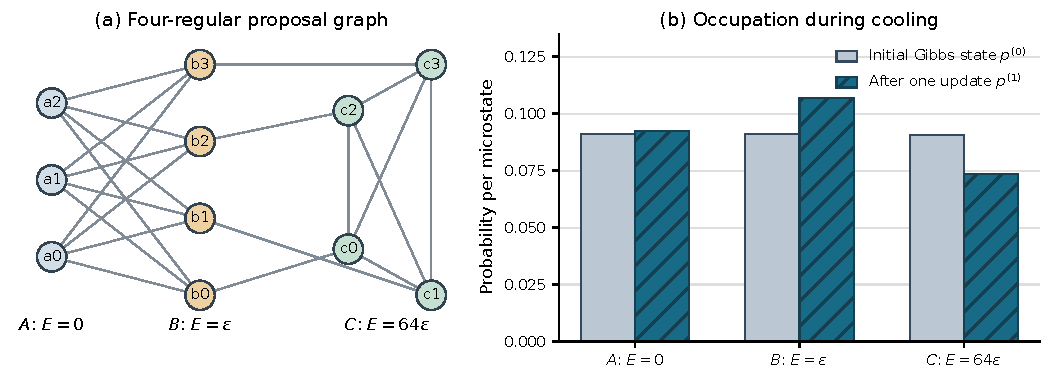
\includegraphics[width=\textwidth]{figures/occupations.pdf}
\caption{(a) The complete proposal graph: 12 $A$--$B$ edges, four matched
$B$--$C$ edges, and six edges inside $C$. Unmarked line crossings are not
vertices, and the drawing is not an energy scale.
(b) Per-microstate probabilities before and after the first update.
The intermediate class $B$ overtakes the lower-energy class $A$.
Class sizes are 3, 4, and 4; heights are not class totals.
The figure uses the specified graph and exact rational data, converted to
floating point only for display, with drawing code drafted using OpenAI
Codex (GPT-6).}
\label{fig:occupations}
\end{figure*}

\section{Uniform stability under energy perturbations}
The violation does not require exact degeneracies. Keep the graph and
temperatures fixed, replace $E_i$ by $E_i+\eps d_i$, and impose
\begin{equation}
|d_i|\leq\delta=\frac1{1000}\qquad\text{independently for every }i.
\label{eq:box}
\end{equation}
Redefine the initial state to be Gibbsian for the perturbed energies at
$\beta_0$. Tildes denote the resulting quantities. We prove the uniform
bounds
\begin{equation}
\widetilde\Act_1>\frac{1003737}{2000000}>\frac12,\qquad
\widetilde{\overline\Act}_2>\frac{8014821}{16000000}>\frac12.
\label{eq:robust-result}
\end{equation}

For clarity write $P_k=P(\beta_k)$ and let $a_k$ be its vector of
escape probabilities. The function $f(q)=(1+e^q)^{-1}$ satisfies
$|f'(q)|\leq 1/4$. An edge energy difference in units of $\eps$ changes
by at most $2\delta$. Summing the off-diagonal changes in a column,
and then including the compensating diagonal change, yields
\begin{equation}
\|\widetilde P_k-P_k\|_1\leq b_k\delta,\qquad
\|\widetilde a_k-a_k\|_\infty\leq\frac{b_k\delta}{2}.
\label{eq:lipschitz}
\end{equation}
Here the matrix norm is the induced $1$-norm. The ratio of perturbed to
unperturbed initial Gibbs weights, after normalization, lies between
$e^{-2b_0\delta}$ and $e^{2b_0\delta}$. Hence
\begin{equation}
\|\widetilde p^{(0)}-p^{(0)}\|_1\leq
\eta_0,\qquad \eta_0=e^{2b_0\delta}-1.
\end{equation}
By stochastic contraction, the $1$-norm distance between the two
distributions after the first update is at most $\eta_0+b_1\delta$.
Using $0\leq a_{k,i}\leq1$ in the activity inner products gives
\begin{align}
|\widetilde\Act_0-\Act_0|&\leq\eta_0+b_1\delta/2,\nonumber\\
|\widetilde\Act_1-\Act_1|&\leq\eta_0+b_1\delta+b_2\delta/2.
\label{eq:activity-error}
\end{align}
These bounds hold on the full perturbation box, without retaining layer
symmetry or truncating a perturbation series.

For the protocol~\eqref{eq:protocol},
\begin{equation}
b_0<\frac1{10000},\qquad b_1<\frac1{32},\qquad b_2<\frac{21}{5}.
\end{equation}
The first two bounds follow from $\log(1+q)<q$ for $q>0$.
For the third, $e^{7/10}>1+7/10+(7/10)^2/2+(7/10)^3/6>2$.
The inequality $e^q-1\leq q/(1-q)$ for $0\leq q<1$ also implies
$\eta_0<1/4000000$. Substitution into
Eq.~\eqref{eq:activity-error} gives
\begin{align}
|\widetilde\Act_1-\Act_1|&<\frac{4263}{2000000},\nonumber\\
|\widetilde{\overline\Act}_2-\overline\Act_2|
&<\frac{17179}{16000000}.
\label{eq:explicit-errors}
\end{align}
Subtracting these error bounds from $63/125$ and $251/500$, respectively,
proves Eq.~\eqref{eq:robust-result}. Thus fully nondegenerate energies
within the stated box also give counterexamples.

\section{Mechanism and scope}
The energy gaps $\eps$ and $63\eps$ respond differently to the first
temperature change. Probability flows from $C$ into $B$ while reverse
$A\to B$ acceptance is still appreciable. The resulting $y>x$, visible in
Fig.~\ref{fig:occupations}, reverses the per-state energy ordering on the
$A$--$B$ edges. The second cooling step makes $B\to A$ strongly favorable.
Together with the remaining $C$ occupation and its internal microstate
jumps, this makes the full correction in Eq.~\eqref{eq:edge} negative.
The construction shows reachability from an exact Gibbs initial state;
merely choosing an arbitrary inverted distribution would not answer the
annealing question.

The equilibrium identity~\eqref{eq:equilibrium} and the explicitly
hypothesized neighborhood-passivity sufficient condition of
Ref.~\cite{LuoDetailed}, Eq.~(41), remain valid. Our result establishes
that regularity, instantaneous detailed balance, a Gibbs initial state,
and monotone cooling do not by themselves enforce the one-half bound.
The same example rules out its two-update averaged counterpart.
The latter matters for the activity substitution in the annealing
performance analysis of Ref.~\cite{LuoLetter}, p.~4, in the discussion
leading to Eq.~(10).

This is a complete finite classical state space, with no state-space
truncation, continuous-time normalization, extra laziness, or infinite-volume
limit. The protocol has two finite temperature changes. The graph is not
a single-spin-flip hypercube. No conclusion follows here for a restriction
to the SK model, to hypercube proposal graphs, or to sufficiently slow
cooling. Nor does failure of one intermediate activity bound alone disprove
the final performance formulas, which involve additional estimates.
We make no assertion of a minimal state count or maximal violation.

\section{Calculation and data availability}
The complete $11\times11$ transition matrices were propagated in rational
arithmetic and compared with a separately implemented sum of synchronous
undirected-edge currents. A further independent implementation enumerated
all $11\times8^2=704$ two-update proposal/acceptance histories, retaining
distinct rejected proposals. All three calculations agree. These are exact
finite calculations, not Monte Carlo estimates.

As a convention check, the equilibrium four-spin periodic ferromagnetic
Ising chain with $H=-J\sum_{i=1}^4s_i s_{i+1}$, $s_5=s_1$, and
$\beta J=(\log2)/2$ gives $Z=41/2$ and acceptance $16/41$ by enumeration.
This agrees with the finite-chain formula of Burovski
\textit{et al.}~\cite{Burovski}, arXiv v2, Appendix, subsection B, Eq.~(24), evaluated
at $L=4$ and $e^{2\beta J}=2$. The value is a substitution into that
published formula, not an additional result of the present work.

OpenAI Codex was used substantively to propose and analyze the construction,
write exact-arithmetic code, and assist source comparisons. The automated
work was directed by fixed requirements for the Glauber rule, Gibbs
initialization, admissible cooling, and exact sign checks. Verification
consisted of the distinct calculations above and analytic error bounds;
AI agreement alone was not used as a sign certificate. The manuscript and
plotting-code preparation used GPT-6. Exact model-version identifiers for
earlier research stages have not been recovered in this draft. Final human
scientific review and confirmation of the disclosure remain pending.

All defining inputs and the scalar sign-verification algorithm are in this
article. The accompanying local source package contains the full propagation,
edge-current and history-enumeration implementations, rational outputs, and
regeneration instructions. No experimental data are used. A public repository
has not been deposited for this draft.

\begin{acknowledgments}
OpenAI Codex (GPT-6 for manuscript preparation) assisted with drafting and
editing the text, bibliography preparation, and presentation code. This
disclosure includes substantive research assistance described above and
does not represent completed human review.
\end{acknowledgments}

\appendix
\section{A short exact sign certificate}
\label{app:certificate}
The following Python 3 code uses only the standard library. It evaluates
the displayed scalar formulas and checks every enclosure in
Table~\ref{tab:exact}. Integer cross multiplication implements comparisons
of \texttt{Fraction} objects, so no numerical precision setting is needed.
\begingroup\footnotesize
\VerbatimInput[fontsize=\footnotesize]{../reproducibility/scalar_certificate.py}
\endgroup

\bibliography{references}
\end{document}
